\documentclass{sig-alternate}
%
%\usepackage{makeidx}  % allows for indexgeneration
%\usepackage[pdftex]{graphicx}\usepackage{graphicx}
\usepackage{float}
\usepackage{subfig}
\usepackage{caption}
\usepackage{graphicx}
\usepackage{amsmath}
\usepackage{algorithm,algorithmicx}
\usepackage{algpseudocode}

\begin{document}
%\normalem


\title{Why so aggresive? Low Extra Delay Backround Traffic (LEDBAT) in WebRTC}

\numberofauthors{3}

\author{
\alignauthor
Riccardo Reale\\
      \affaddr{Peerialism AB}\\
      \affaddr{Stockholm, Sweden}\\
      \email{mikael@peerialism.com}
\alignauthor
Anton Blomberg\\
      \affaddr{Stockholm University}\\
      \affaddr{Stockholm, Sweden}\\
      \email{anton@su.se}
\alignauthor
Roberto Roverso\\
      \affaddr{Peerialism AB}\\
      \affaddr{Stockholm, Sweden}\\
      \email{roberto@peerialism.com}
}

\newcommand{\mysec}[1]{\vspace*{-0.0cm}\section{#1}}
\newcommand{\mysubsec}[1]{\vspace*{-0.0cm}\subsection{#1}\vspace*{0cm}}
\newcommand{\mysubsubsec}[1]{\vspace*{-0.0cm}\subsubsection{#1}\vspace*{0cm}}
\newcommand{\mypar}[1]{\vspace*{-0cm}\paragraph{#1}\vspace*{0cm}}

\maketitle
%\vspace*{-1cm}

\begin{abstract}

In this paper, we present what is, to the best of our knowledge, the first implementation
of LEDBAT for the WebRTC framework. In particular, we detail how we integrated the
protocol in the WebRTC stack in a way that features such as relialibility, in-order
delivery and encryption could also be applied to LEDBAT transfers and not only to
the existing transfer protocol (SCTP). We also include preliminary results of this effort
that show the correct functioning of our implementation.
\end{abstract}

\category{C.2.2}{Computer-Communication Networks}{Network Protocols}
\category{C.2.4}{Computer-Communication Networks}{Distributed Systems}
\terms{Experimentation, Performance, Measurement}
\keywords{LEDBAT, WebRTC, Peer-to-peer}

\mysec{Introduction}
% WebRTC general 
Recently, WebRTC has been steadily gaining popularity fueled by the inclusion in most of
the browsers on the market. The WebRTC standard mandates the multimedia and peer-to-peer
connectivity stacks for real-time services, once provided by external plugins, to be built
directly into the browser. That means that the functionality of those stacks, such as
video acquisition, noise cancelling and NAT traversal, is directly available through
Javascript and HTML5 APIs. Although WebRTC has been mainly designed as a framework to
facilitate video and audio conferencing, it does include support for building other types
of peer-to-peer applications, such as CDN accellerators~\cite{peerCDN} and video streaming
platforms~\cite{nurminen2013p2p}. This feature is provided through the DataChannel
abstraction, which allows the transfer of arbitrary data over encrypted connections
established with WebRTC's NAT traversal facilities. The DataChannel API make use of the
Stream Control Transfer protocol (SCTP)~\cite{sctp} protocol in order to manage data
transfers. SCTP is message-oriented protocol and provides a variety of options on data
transfer to accomodate the needs of different types of applications. When setting up a
DataChannel, WebRTC applications may choose in- or out-of-order delivery, reliable or
unreliable delivery and have a specific priority level on the channel. Regarding
congestion control, the latest version of SCTP included in WebRTC make use of the same
congestion control found in H-TCP~\cite{htcp}. The main characteristic of H-TCP is that it
delivers the same priority as TCP in low bandwidth networks while trying to exploit better
capacity large bandwidth links always compared to TCP.

% Why LEDBAT is important
Although the DataChannel implementation currently provides very useful features, it lacks
a fundamental component that is low priority traffic. This is usually provided in P2P
network stacks by a delay-based congestion protocol such as LEDBAT~\cite{ledbat}. LEDBAT
achieves low priority behavior by completely yeilding to other TCP traffic on the same
network and by keeping the delay on a link fixed to a low and constant target. By adopting
such protocol, data-intensive applications such as Bittorrent avoid disrupting both
TCP-based web browsing and low delay VoIP applications. Low priority traffic is also a
vital requirement for other types of applications, such as streaming
platfroms~\cite{smoothcache}\cite{roberto-thesis}.

% What we did 
In this paper, we present what is, to the best of our knowledge, the first implementation
of LEDBAT for the WebRTC framework. In particular, we detail how we integrated the
protocol in the WebRTC stack such that features like relialibility, in-order delivery and
encryption could also be applied to LEDBAT and not only to SCTP. We also include
preliminary results of this effort that show the correct functioning of our
implementation.

% Open source
The implementation is open-source and can be found at~\cite{}. We hope that, by adding
LEDBAT to WebRTC, we will enable a new class of data-intensive applications to be
developed on Javascript that are pluginless and can cohexist with standard web browsing
and the typical application of WebRTC, that is conferencing.


% General video
% As of December 2013, video streaming constitutes $29\%$ of the Internet traffic worldwide
% and it is expected to grow four times in volume in the next $3$ years~\cite{cisco}.  Given
% these growth figures, it is unclear if current Content Delivery Network (CDN) technology
% will be able to efficiently support such large amount of traffic in a cost-effective manner.

% % Why p2p is good
% Peer-to-peer (P2P) technology has been proposed as a complement to standard CDN
% infrastructure to greatly reduce distribution costs and improve quality of user experience
% for viewers~\cite{cdn-p2p}. In an industrial setting, we already find instances of such
% P2P platforms in Akamai's NetSession~\cite{netsession} and Adobe RTMFP
% platform~\footnote{http://labs.adobe.com/technologies/cirrus/}, a part of the Adobe Flash plugin.

% %Adoption
% However, up until now, adoption of P2P technology for content distribution has been
% hindered by the fact that available platforms require the installation of client-side
% software, as in NetSession, or a browser plugin, as in RTMFP.

% % Even better if p2p streaming in browser: WebRTC and frictionless deployment
% Fortunately, with the advent of the WebRTC standard, this limitation is bound to
% disappear. WebRTC defines a set of APIs, to be included in all browsers, that are designed
% to facilitate the development of browser-based real-time P2P applications. As a
% consequence, WebRTC completely removes the need for third-party plugins or client-side
% software and allows frictionless deployment of new P2P-based services as Javascript
% applications. In order to achieve that goal, functionalities necessary to real-time
% applications, such as NAT Traversal and real-time transport protocols, have been built
% directly into the browser. Currently, stable WebRTC implementations exists in three major
% browsers, that is Chrome, Firefox and Opera.

% In this work, we present a browser-based distributed caching application, called
% \textit{Hive.js}, that leverages a P2P overlay network created with WebRTC to
% significantly reduce the load on traditional CDNs. We implement our solution considering
% the realities of the streaming market by adopting adaptive HTTP streaming and,
% specifically, MPEG-DASH~\footnote{http://dashif.org/mpeg-dash/} as streaming protocol of
% choice. DASH is already widely embraced by providers, such as YouTube, and it is expected
% to become the de-facto standard for the distribution of video content on the Internet.

% Hive.js is the plugin-less version of the commercial P2P streaming application Hive
% Streaming\footnote{www.hivestreaming.com}~\cite{roverso2013http}. Initial results obtained
% in a realistic yet controlled environment show that Hive.js, albeit still in a prototype
% phase, is able to significantly offload traditional CDN while maintaining a good level of
% quality of user experience.

% The current version of Hive.js is open source and can be found at~\cite{hive-repo}.

% What is DASH
% The DASH standard aims at defining a protocol for the
% delivery of video and audio streams over the Internet using HTTP as transport. HTTP
% streaming has become the de-facto standard for the content delivery business for
% large-scale disitrbution. 
% The use of HTTP has several benefits: i) distributing HTTP
% content over CDNs is cheap and efficient, ii) it is firewall friendly, iii) HTTP provision
% and distribution technology is mature and well-understood. 
% DASH also makes use of adaptive bitrate technology which adapts to the amount of bandwdith
% and computational power available at the host. This is to support different platforms
% including computers, tablets and smart phones. DASH is an effort to superseed current
% proprietary HTTP-based streaming protocols such as HLS, Smooth Streaming and HDS that are
% based on the same concepts but are not interoperable.


% \mysec{Background and Related Work} 

% The WebRTC standard mandates the multimedia and peer-to-peer connectivity stacks for
% real-time services, once provided by external plugins, to be built directly into the
% browser. The functionality of those stacks, such as video acquisition or noise cancelling,
% are made available to developers through HTML5 APIs. The most prominent functionality for
% our use-case is NAT traversal with the inclusion of
% libjingle\footnote{https://developers.google.com/talk/libjingle} which implements the ICE,
% STUN and TURN protocols.  As a consequence, when building a WebRTC application, all
% complex NAT traversal operations are entrusted to the browser itself and hidden from the
% developer. However, as a design choice, WebRTC does not provide a signalling protocol for
% discovering and managing nodes in the peer-to-peer network, but rather assumes that
% implementers either make use of pre-existing protocols (SIP, Jingle, etc.) or provide
% their own. Another important feature recently added to the standard is the DataChannel
% abstraction that allows the transfer of arbitrary data. Earlier WebRTC communication was
% limited to video conferencing or VoIP traffic. Datachannel allow the implementation of
% generic P2P applications on top of WebRTC, such as peer-to-peer streaming. The DataChannel
% APIs make use of the SCTP protocol. SCTP is a message-oriented protocol that provides
% configurable reliability of transfers and TCP-friendliness. 

% % Background DASH - general - maybe we can move this to intro? 
% Besides WebRTC, in our platform, we make use of a Javascript-based player for DASH.
% % Background DASH - more detailed
% DASH defines a protocol for the delivery of video and audio streams over the Internet
% using HTTP as transport. It also makes use of the adaptive bitrate mode of operation which
% adapts to the amount of bandwidth and computational power available at the host in order
% to support different bandwidth scenarios and types of devices, such as phones, tablets and
% PCs. DASH is an effort to superseed current proprietary HTTP-based streaming protocols
% such as HLS, Smooth Streaming and HDS that are based on the concept of HTTP streaming and
% adaptive bitrate switching but are not interoperable.

% DASH is based on a pull-model, where the player requests content chunks, that is
% \textit{fragments}, from the CDN using HTTP at the pace it deems suitable. The same
% fragment of content exists in many versions, that is one for each bitrate. The choice of
% which bitrate to retrieve and play is left to the player. The bitrates available, the
% duration of the fragments and other playback-specific information is provided in a metadata
% descriptor, called the \textit{manifest}, that is passed as input to the player upon the
% start of the playback. The DASH Forum provides a reference implementation of a player for
% DASH that is implemented in Javascript over HTML5 APIs. The player makes use of the W3C
% Media Source Extensions to allow client-side scripts to parse manifests, request fragments
% and apply bitrate switching logic while leaving the tasks of content decoding and
% rendering to the browser.

% % P2P layer
% In order to stream DASH-generated content over a peer-to-peer overlay created with WebRTC,
% we employ a Distributed Caching approach. Each fragment retrieved by a peer is stored and
% made available for later retrieval by its neighbours. In this way, when a player requests a
% fragment, peers avoid getting fragments that are available at their neighbours from the
% source, but they rather resort to P2P. This significantly decreases the load on
% the CDN infrastructure, and therefore the cost of distribution. Previous literature on the
% subject has shown that this method is particularly effective for the task of distributing
% adaptive HTTP streaming content at large scale~\cite{smoothcache}. In the same work, it
% has also been shown that classical P2P streaming approaches, such as~\cite{newcool}, are
% not applicable for adaptive bitrate HTTP streaming.

% Concerning browser-based P2P content distribution, we find very little related work. Few
% address the more general problem of optimising the distribution of generic web content
% rather than video. In Maygh~\cite{maygh}, authors present a system which uses both WebRTC
% and the RTMFP~\cite{RTMFP} framework for peer-to-peer operations. The authors show that
% Maygh can offload up to $75\%$ of traffic from the CDN, considering a standard web-portal
% scenario. Two commercial offerings PeerCDN~\cite{peerCDN} and Swarmify~\cite{swarmify} try
% to achieve the same goal using only WebRTC. Although relevant to content distribution, the
% aforementioned systems are not specifically designed for streaming and it is unclear
% whether they would yield any particular advantage in that use case.

% Regarding browser-based P2P streaming, to the best of our knowledge, the only related work
% is~\cite{nurminen2013p2p}. The paper briefly outlines the architecture of a live streaming
% platform based on WebRTC which employs a structured overlay network (DHT) for locating
% video fragments. However, no implementation details or evaluation is provided.
% Consequently, to the best of our knowledge, we are the first to develop and evaluate a
% fully functional browser-based peer-to-peer platform that does not require any plugin and
% it is specifically designed for the distribution of video content.

\begin{figure}[t]
  \centering
    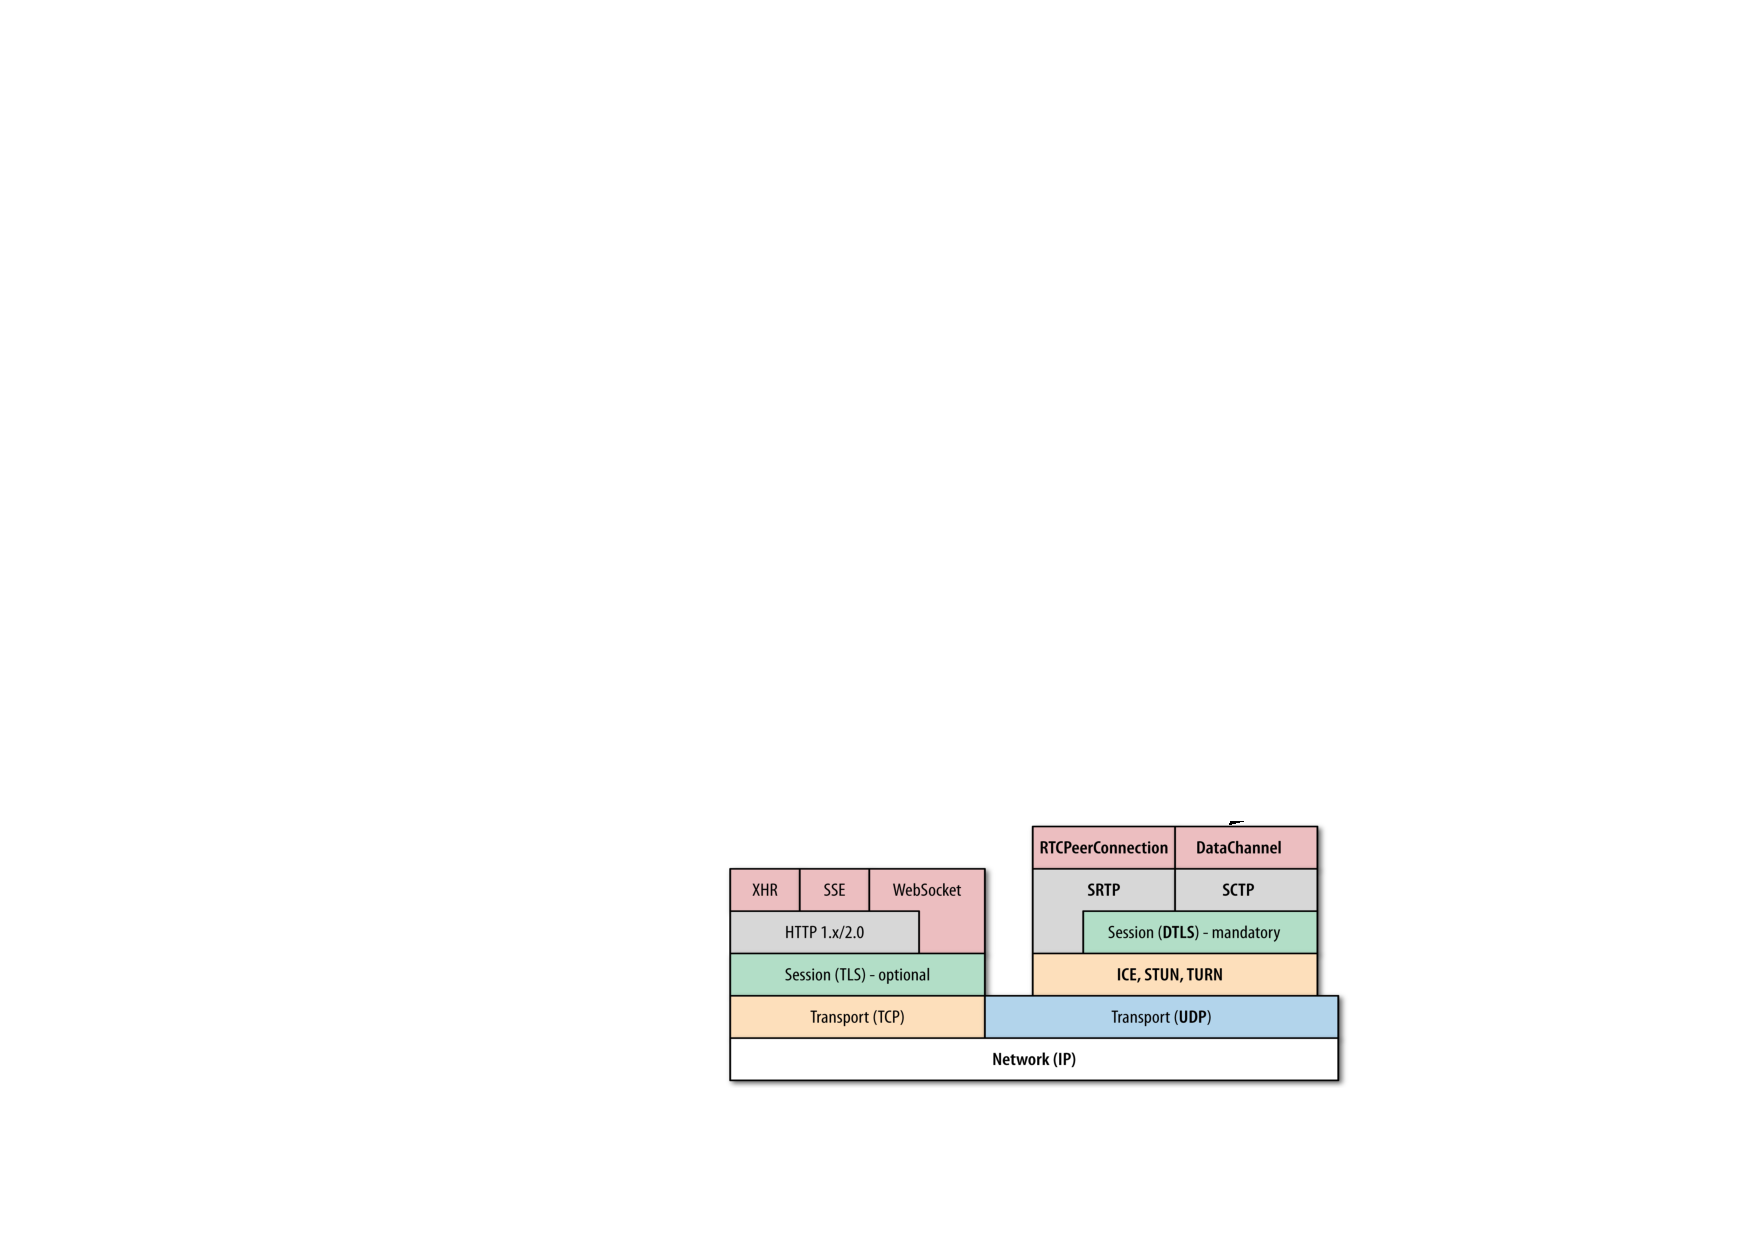
\includegraphics[width=0.46\textwidth]{figs/architecture}
\vspace*{-0.38cm}
	\caption{Architecture of Node} \label{fig:architecture}
\vspace*{-0.4cm}
\end{figure}

\mysec{LEDBAT in WebRTC}
\label{sec:architecture}

% % General
% The design of our system is based on a Distributed Caching model that works as follows:
% upon a content fragment request from the DASH player, the distributed cache tries to
% timely retrieve the data requested from other peers in the overlay. If a fragment cannot
% be retrieved from any other peer on time, the agent downloads it from the source of the
% stream, i.e. the CDN. By falling back to the source, we make sure that all fragments are
% delivered to the player even if the overlay network cannot retrieve such fragments,
% thereby guaranteeing the desired level of QoE.

% Regarding the overlay, we create a random graph between all peers watching a stream. Each
% node selects a fixed number of neighbours and connects to them. Periodically, the peer
% randomly selects one of its neighbours and terminates the connection to it. After that, it
% connects to a new peer chosen at random from a list of potential neighbours that is
% provided by a central tracker.

% % Implementation
% In Figure~\ref{fig:architecture}, we show the architecture of our application. We make use
% of the reference DASH player implementation and a set of scripts that implement our
% caching abstraction, the \textit{Distributed Cache} layer in the figure. Upon the load of
% the web page, the DASH player is instructed to load a stream. After that, the
% \textit{Discovery} component initiates a connection to a well-known tracker address using
% the WebSocket Client APIs. 
% % This is because WebRTC does not provide any means of
% % discovering new nodes but that task is left to the application developer as the
% % functionality could be developed in several different ways. 
% Once a successful connection is established, the nodes asks for a list of nodes to connect
% to. The tracker returns a random subset from all peers watching the same stream.

% At this point, the peer attempts to establish a WebRTC DataChannel connection with the
% returned peers using the WebRTC's NAT Traversal utilities. If a direct connection could be
% achieved, that is without the need of a relay, the \textit{Peer} component stores
% information about the neighbour in a dedicated \textit{Channel} instance. The Channel
% module interacts with the WebRTC DataChannel API to send and receive data from/to the
% corresponding peer. We choose a configuration of the DataChannel that provides reliable
% message-oriented transfer of data over the SCTP protocol. However, the implementation of
% SCTP in the browsers does not allow the transmission of arbitrarily long messages. Since
% video fragments can be fairly large, in the order of megabytes, we implement a transport
% protocol, in the sub-module \textit{P2P transport}, which transfers fragments in smaller
% chunks of fixed size. The integrity of each chunk is verified by the receiver using a hash
% of the fragment that is sent together with the data.


% % Each chunk a hash of the content calculated on the fly. This is used to check the
% % integrity of the information once it reaches the destination. If the check is successful,
% % an acknowledgement is sent to the sender, which in turn sends the next chunk of fragment
% % data, if any. If no chunk is left, the transfer is terminated and the sender notified. The
% % protocol is implemented in the sub-module \textit{P2P transport}.

% The transfer of a fragment is triggered by a request from the DASH player. The player is
% designed in a modular fashion, consequently each module can be easily replaced with a new
% implementation. In order to provide our distributed caching mechanism, we provide an
% alternative implementation of the \textit{Fragment Loader} module. We instrument the
% module to forward fragment requests to the Peer component if a fragment is present at the
% Peer's neighbours. If the fragment is not available, the content is requested to the
% source of the stream with a XMLHttpRequest through the \textit{XHR} interface provided
% by the browser, as it would happen in the standard implementation of the Fragment Loader.

% Upon a successful retrieval of a fragment, either from the source or the overlay, a peer
% stores the fragment data in memory using the \textit{Cache} module and then it sends a
% Have notification to all its neighbours. On the receiving end, a peer inserts the
% information about which fragment is available at which neighbour in the \textit{Index}
% component.

% % P2P transport
% For the actual retrieval of the fragment from the overlay, we follow a pull-based
% approach. Once the player issues a fragment request, the peer checks if it is present in
% the Index component. If so, the Peer module chooses a neighbour from all possible peers
% uniformly at random and sends a fragment request to it. If the fragment is retrieved
% successfully, the Peer component delivers the data to the DASH player. Otherwise, if the
% transfer was interrupted or it timed out, the fragment is retrieved from the source of the
% content. By falling back to the source, we guarantee that all fragments are delivered to
% the player even if the overlay network cannot retrieve such fragments, thereby preventing
% interruptions to the playback and loss of QoE.

\mysec{Preliminary results and demo}

% \mysec{Evaluation}

% \begin{figure*}[t]
%   \centering
%   \subfloat[Transferred data]{
%     \includegraphics[width=0.33\textwidth]{figs/seeder_transfers_p2p_src}
%   }
%  \subfloat[Savings]{
%     \includegraphics[width=0.33\textwidth]{figs/savings}
%   }
%   \subfloat[Buffer size]{
%     \includegraphics[width=0.33\textwidth]{figs/buffer_size}
%   }
%   \caption{
%   \label{fig:results}
%   Results from both the single-seeder and swarm with an increasing number of peers.
%   }
% \end{figure*}


% In this evaluation, we provide validation of the correct functioning of our platform and
% test the limits of the same. 

% %Specifically, the goal of our investigation is to analyse: i)
% %the maximum upload contribution that a peer can provide to the overlay, ii) the 

% %\mysubsec{Experiment setup} 

% In our experiments, each node executes a headless instance of Google Chrome
% $33.0.1750.149$ on Linux using XFVB as output interface. Each instance runs on a dedicated
% Microsoft Azure dual-core Virtual Machine with 3GB memory and 200Mbps of available
% bandwidth capacity. Upon the joining of a node, Chrome is instructed to load a static test
% page that consists of the DASH player and HCache, as explained previously. We use version
% $1.1.2$ of the DASH reference player, which was the latest version of the player at the
% time of writing. We let the player watch a production video stream provided by
% Envivo\footnote{http://dash.edgesuite.net/envivio/dashpr/clear/Manifest.mpd} in a single
% bitrate configuration of 2Mbps for video, with 4 second segments, and 56 kbps for
% audio. As in all adaptive HTTP streaming players, a buffer is kept by the player to
% compensate for temporary disruptions in the delivery of the stream caused by, for
% instance, network congestion and temporary loss of connectivity. For the chosen
% stream, the DASH player keeps a buffer of up to 10 seconds.

% % Tracker
% Our testbed also includes a central Tracker, implemented in Python, which serves both as a
% discovery facility, which the peers periodically query to obtain a list of potential
% neighbours, and as broker for WebRTC connection setups.

% % Metrics
% We conducted a number of initial experiments in a controlled environment to assert the
% feasibility of our approach. The testbed constituted of $30$ dual-core machines with high
% bandwidth capacity (200Mbps). For our tests, we used the $1.1.2$ version of the DASH
% reference player, augmented with Hive.js, and we played a Video-On-Demand production
% stream with 2Mbps of bitrate. In this scenario, Hive.js managed to offload $95\%$ of the
% traffic from the CDN and provide the same quality of user experience as a CDN in terms of
% latency.

% In the demo, we will show our platform running on a number of computers on-site and we
% will allow participants to join the demo session from their phone, tablet or laptop. We
% will also provide extensive visualization of the live P2P overlay data and performance
% metrics both from the live sessions and pre-recorded ones.

% Finally, we provide a deployment of our platform at~\cite{hive-repo} for any
% interested party to experiment with.

% In our experiments, we observe two main metrics: the player's average buffer size and the
% amount of savings towards the source of the stream. Monitoring the buffer size is a way to
% measure quality of user experience (QoE) provided by the platform. The rationale is that,
% if a player manages to maintain a sufficiently large buffer by retrieving data in time,
% either from P2P or the CDN, the playback is less likely to be disrupted due to network
% issues.

% The savings instead are a measure of the performance of the systems as a whole and they
% indicate how much HCache managed to offload the CDN. Savings are calculated as the total
% amount of data retrieved from P2P during an experiment over the total amount of transfered
% data.

% In our experiments, we use two different scenarios. The first one, which we call
% \textit{seeder-only}, has the purpose of showing the maximum upload contribution that a
% peer can provide to the overlay. It is constructed in the following way: a peer (seeder)
% plays the entire video. After it finishes, the other peers (leechers) join uniformly at
% random in a 60 seconds window and start watching. Upon start, leechers receive
% notifications (Haves) from the seeder indicating which fragments the seeder has
% downloaded. However, in this experiment, we instruct leechers not to issue Haves
% themselves. As a consequence, there is no inter-leecher P2P traffic.

% In the second scenario, which we call the \textit{swarm} scenario, we aim at analysing the
% performance of the platform as a whole. For that, we remove the seeder and we let all
% peers behave normally, thus allowing peer-to-peer communication between leechers. Again,
% the peers join uniformly at random in a 60 seconds window. In both scenarios, peers watch
% a video lasting $4.2$ minutes. Each experiment is repeated 3 times and we show max, min
% and average.

% %To make the experiments more predictable, we have also
% %modified the player slightly to only allow a single concurrent request per fragment type
% %(audio and video).

% \mypar{Seeder-only}

% Figure \ref{fig:results} a) shows the amount of data (bytes) transferred by
% all peers in the seeder-only scenario from the seeder (P2P) and the source (SRC) with
% increasing number of nodes. The amount of data transferred for a single peer is fixed and
% it is the size of the video (60MB). We observe that for more than $20$ peers, the leechers cannot retrieve data
% from the seeder fast enough. Thus, they start to compensate the poor throughput of the
% seeder by downloading from the source. We also confirm that the total amount of
% transferred data grows linearly with the number of viewers. Figure~\ref{fig:results} b)
% shows the same trend, where the savings start to drop after $20$ leechers.

% In Figure~\ref{fig:results} c) we show the average buffer size across all peers with
% increasing number of peers. There we can observe that, when the seeder becomes overloaded,
% the average buffer size at the leechers decreases (around $10$ peers), indicating that some leechers are
% experiencing disruptions in the playback. From this we derive that a single seeder cannot
% serve more than $10$ peers without impacting the overall QoE.


% %That is due to the fact that the time
% %it takes to download fragments from the seeder also increases with the number of peers.
% %However, for more than $10$ peers, some leechers start to experience disruptions in the
% %playback.


% %some starts to experience since they compensate by
% %going to the source which can serve the fragments within the deadline. From this we derive
% %that a single seeder cannot serve more than $12$ leechers without impacting the overall
% %QoE.


% %\begin{figure}[t]
% %  \centering
% %    \includegraphics[width=0.5\textwidth]{figs/seeder_transfers_p2p_src}
% %	\caption{Total data transferred of p2p vs. source traffic.}
% %  \label{fig:seeder_transfers_p2p_src}
% %\end{figure}

% \mypar{Swarm scenario}

% In comparison to the seeder-only scenario, in the swarm scenario the average buffer size
% remains stable over time, as depicted in Figure~\ref{fig:results} c).  This is because,
% when peers can retrieve data from each other, the load is balanced over all nodes,
% effectively avoiding a single seeder to become overloaded. As peers join they also contribute
% to the overall capacity of the system. This effect is also observed in the savings, which
% increase logarithmically with the number of viewers (Figure~\ref{fig:results} b)).  Both
% b) and c) indicates that the fragment download time on a leecher is within the deadline,
% and as a result not affecting the QoE.

% % Figure~\ref{fig:savings} shows that when the
% % seeder capacity is reached more peers accesses the source which leads to reduced savings.
% % For the P2P case, the data fetched from the source is constant which increases the savings
% % when the number of viewers increase.

% %On a high level, the buffer size indicates the quality of experience for a user. If the
% %buffer goes towards zero, the player stops and 


% % \begin{figure}[t]
% %   \centering
% %     \includegraphics[width=0.5\textwidth]{figs/buffer_size}
% % 	\caption{The average buffer size (in seconds) for an increasing number of viewers.}
% %   \label{fig:buffer_size}
% % \end{figure}

% % \begin{figure}[t]
% %   \centering
% %     \includegraphics[width=0.5\textwidth]{figs/savings}
% % 	\caption{The savings (P2P over source traffic) for an increasing number of viewers.}
% %   \label{fig:savings}
% % \end{figure}
 
% \mysec{Conclusion} 

% We have presented HCache, a browser-based plugin-less video distribution solution layered
% over the WebRTC peer-to-peer APIs. Our platform utilizes a distributed caching approach
% that is designed to transport adaptive HTTP streaming content, and specifically
% MPEG-DASH. Initial results obtained by evaluating HCache in a controlled environment show
% that our solution is viable and does not sacrifice quality of user experience while
% producing significant savings towards the source of the stream, that is the CDN.

% As future work, we plan to continue investigating this approach in more realistic
% scenarios with large number of nodes and heterogeneous network environments.

%\footnotesize

%\footnotesize
\bibliographystyle{abbrv}
\bibliography{main}


\end{document}
